\documentclass{report}
\usepackage{luatexja} % LuaTeXで日本語を使うためのパッケージ
\usepackage{luatexja-fontspec} % LuaTeX用の日本語フォント設定
% lualatex main && upmendex -r -c -s main.ist -g main && lualatex main  

% --- 数学関連 ---
\usepackage{amsmath, amssymb, amsfonts, mathtools, bm, amsthm} % 基本的な数学パッケージ
\usepackage{type1cm, upgreek} % 数式フォントとギリシャ文字k
\usepackage{physics, mhchem} % 物理や化学の記号や式の表記を簡単にする

% --- 表関連 ---
\usepackage{multirow, longtable, tabularx, array, colortbl, dcolumn, diagbox} % 表のレイアウトを柔軟にする
\usepackage{tablefootnote, truthtable} % 表中に注釈を追加、真理値表
\usepackage{tabularray} % 高度な表組みレイアウト

% --- グラフィック関連 ---
\usepackage{tikz, graphicx} % 図の描画と画像の挿入
% \usepackage{background} % ウォーターマークの設定
\usepackage{caption, subcaption} % 図や表のキャプション設定
\usepackage{float, here} % 図や表の位置指定

% --- レイアウトとページ設定 ---
\usepackage{fancyhdr} % ページヘッダー、フッター、余白の設定
\usepackage[top = 20truemm, bottom = 20truemm, left = 20truemm, right = 20truemm]{geometry}
\usepackage{fancybox, ascmac} % ボックスのデザイン

% --- 色とスタイル ---
\usepackage{xcolor, color, colortbl, tcolorbox, ulem} % 色とカラーボックス
\usepackage{listings, jvlisting} % コードの色付けとフォーマット
\definecolor{apsblue}{HTML}{2d3092}

% --- 参考文献関連 ---
% \usepackage[style=phys, backend=biber]{biblatex}
\usepackage[backend=biber, sortcites=true, style=phys, doi=false]{biblatex}
\usepackage{usebib} % 参考文献の管理と挿入
\usepackage{url} % URLとリンクの設定
\usepackage[colorlinks=true, linkcolor=apsblue, citecolor=apsblue, urlcolor=apsblue]{hyperref}

% --- その他の便利なパッケージ ---
\usepackage{footmisc} % 脚注のカスタマイズ
\usepackage{multicol} % 複数段組
\usepackage{comment} % コメントアウトの拡張
\usepackage{siunitx} % 単位の表記
\usepackage{docmute, needspace}
\usepackage{makeidx}

% \renewbibmacro*{title}{%
%   \printtext[title]{\printfield[titlecase]{title}.\addspace}%
% }
% --- 定理スタイルと数式設定 ---
\theoremstyle{definition} % 定義スタイル
\numberwithin{equation}{chapter} % 式番号をサブセクション単位でリセット

% --- その他の設定 ---
\allowdisplaybreaks % 数式の途中改ページ許可
\newcolumntype{t}{!{\vrule width 0.1pt}} % 新しいカラムタイプ
\newcolumntype{b}{!{\vrule width 1.5pt}} % 太いカラム
\UseTblrLibrary{amsmath, booktabs, counter, diagbox, functional, hook, html, nameref, siunitx, varwidth, zref} % tabularrayのライブラリ
\setlength{\columnseprule}{0.4pt} % カラム区切り線の太さ
% \captionsetup[figure]{font = bf} % 図のキャプションの太字設定
% \captionsetup[table]{font = bf} % 表のキャプションの太字設定
% \captionsetup[lstlisting]{font = bf} % コードのキャプションの太字設定
% \captionsetup[subfigure]{font = bf, labelformat = simple} % サブ図のキャプション設定
\setcounter{secnumdepth}{4} % セクションの深さ設定
\newcolumntype{d}{D{.}{.}{5}} % 数値のカラム
\newcolumntype{M}[1]{>{\centering\arraybackslash}m{#1}} % センター揃えのカラム
\DeclareMathOperator{\diag}{diag}
\everymath{\displaystyle} % 数式のスタイル

\setcounter{tocdepth}{0} % 目次の深さ
% \makeatletter
% \@addtoreset{equation}{chapter} % セクションごとに式番号をリセット
% \makeatother

\newcommand{\braketg}{\braket{\r{g}}}

% \DeclareFieldFormat{journal+issuetitle}{%
%   \iffieldundef{doi}
%     {\printfield{journal}%
%      \setunit*{\addspace}%
%      \printfield{volume}%
%      \setunit*{\addcomma\space}%
%      \printfield{pages}}
%     {\href{https://doi.org/\thefield{doi}}%
%      {\printfield{journal}%
%       \setunit*{\addspace}%
%       \printfield{volume}%
%       \setunit*{\addcomma\space}%
%       \printfield{pages}}}}

% \DeclareFieldFormat{year}{(\printfield{year})}
\DeclareSourcemap{
  \maps[datatype=bibtex, overwrite=true]{
    \map{
      \step[
        fieldsource=journal,
        match=\regexp{Physical\sReview\sLetters},
        replace={Phys. Rev. Lett.}
      ]
      \step[
        fieldsource=journal,
        match=\regexp{Physical\sReview\sA},
        replace={Phys. Rev. A}
      ]
      \step[
        fieldsource=journal,
        match=\regexp{Physical\sReview\sB},
        replace={Phys. Rev. B}
      ]
      \step[
        fieldsource=journal,
        match=\regexp{Physical\sReview\sC},
        replace={Phys. Rev. C}
      ]
      \step[
        fieldsource=journal,
        match=\regexp{Physical\sReview\sD},
        replace={Phys. Rev. D}
      ]
      \step[
        fieldsource=journal,
        match=\regexp{Physical\sReview\sE},
        replace={Phys. Rev. E}
      ]
      \step[
        fieldsource=journal,
        match=\regexp{Physical\sReview\sX},
        replace={Phys. Rev. X}
      ]
      \step[
        fieldsource=journal,
        match=\regexp{Reviews\sof\sModern\sPhysics},
        replace={Rev. Mod. Phys.}
      ]
      \step[
        fieldsource=journal,
        match=\regexp{Journal\sof\sApplied\sPhysics},
        replace={J. Appl. Phys.}
      ]
      \step[
        fieldsource=journal,
        match=\regexp{Applied\sPhysics\sA},
        replace={Appl. Phys. A}
      ]
      \step[
        fieldsource=journal,
        match=\regexp{Applied\sPhysics\sB},
        replace={Appl. Phys. B}
      ]
      \step[
        fieldsource=journal,
        match=\regexp{Applied\sPhysics\sLetters},
        replace={Appl. Phys. Lett.}
      ]
      \step[
        fieldsource=journal,
        match=\regexp{Review\sof\sScientific\sInstruments},
        replace={Rev. Sci. Instrum.}
      ]
      \step[
        fieldsource=journal,
        match=\regexp{Nature},
        replace={Nature}
      ]
      \step[
        fieldsource=journal,
        match=\regexp{Science},
        replace={Science}
      ]
      \step[
        fieldsource=journal,
        match=\regexp{Nature\sPhysics},
        replace={Nat. Phys.}
      ]
      \step[
        fieldsource=journal,
        match=\regexp{Nature\sCommunications},
        replace={Nat. Commun.}
      ]
      \step[
        fieldsource=journal,
        match=\regexp{Scientific\sReports},
        replace={Sci. Rep.}
      ]
      \step[
        fieldsource=journal,
        match=\regexp{Journal\sof\sPhysics\sA:\sMathematical\sand\sTheoretical},
        replace={J. Phys. A: Math. Theor.}
      ]
      \step[
        fieldsource=journal,
        match=\regexp{Journal\sof\sPhysics\sB:\sAtomic,\sMolecular\sand\sOptical\sPhysics},
        replace={J. Phys. B: At. Mol. Opt. Phys.}
      ]
      \step[
        fieldsource=journal,
        match=\regexp{Journal\sof\sPhysics:\sCondensed\sMatter},
        replace={J. Phys.: Condens. Matter}
      ]
      \step[
        fieldsource=journal,
        match=\regexp{Annalen\sder\sPhysik},
        replace={Ann. Phys.}
      ]
      \step[
        fieldsource=journal,
        match=\regexp{Europhysics\sLetters},
        replace={Europhys. Lett.}
      ]
      \step[
        fieldsource=journal,
        match=\regexp{New\sJournal\sof\sPhysics},
        replace={New J. Phys.}
      ]
      \step[
        fieldsource=journal,
        match=\regexp{Physics\sLetters\sA},
        replace={Phys. Lett. A}
      ]
      \step[
          fieldsource=journal,
          match=\regexp{Physics\sLetters\sB},
          replace={Phys. Lett. B}
      ]
      \step[
          fieldsource=journal,
          match=\regexp{Optical\sand\sQuantum\sElectronics},
          replace={Opt. Quantum Electron.}
      ]
    }
  }
}
\newcommand{\inner}[2]{\left\langle #1, #2 \right\rangle}
\renewcommand{\figurename}{図}
\renewcommand{\i}{\mathrm{i}} % 複素数単位i
\renewcommand{\laplacian}{\grad^2} % ラプラシアンの記号
\renewcommand{\thesubfigure}{(\alph{subfigure})} % サブ図の番号形式
\newcommand{\m}[3]{\multicolumn{#1}{#2}{#3}} % マルチカラムのショートカット
\renewcommand{\r}[1]{\mathrm{#1}} % mathrmのショートカット
\newcommand{\e}{\mathrm{e}} % 自然対数の底e
\newcommand{\Ef}{E_{\mathrm{F}}} % フェルミエネルギー
\renewcommand{\c}{\si{\degreeCelsius}} % 摂氏記号
\renewcommand{\d}{\r{d}} % d記号
\renewcommand{\t}[1]{\texttt{#1}} % タイプライタフォント
\newcommand{\kb}{k_{\mathrm{B}}} % ボルツマン定数
\renewcommand{\epsilon}{\varepsilon}
\newcommand{\fullref}[1]{\textbf{\ref{#1} \nameref{#1}}}
\newcommand{\reff}[1]{{図\ref{#1}}} % 図参照のショートカット
\newcommand{\reft}[1]{{表\ref{#1}}} % 表参照のショートカット
\newcommand{\refe}[1]{{式\eqref{#1}}} % 式参照のショートカット
\newcommand{\refp}[1]{{コード\ref{#1}}} % コード参照のショートカット
\renewcommand{\lstlistingname}{コード} % コードリストの名前
\renewcommand{\theequation}{\thesection.\arabic{equation}} % 式番号の形式
\renewcommand{\footrulewidth}{0.4pt} % フッターの線
\newcommand{\mar}[1]{\textcircled{\scriptsize #1}} % 丸囲み文字
\newcommand{\combination}[2]{{}_{#1} \mathrm{C}_{#2}} % 組み合わせ
\newcommand{\thline}{\noalign{\hrule height 0.1pt}} % 細い横線
\newcommand{\bhline}{\noalign{\hrule height 1.5pt}} % 太い横線
\renewcommand{\appendixname}{付録}

\ExecuteBibliographyOptions{
  sorting=none, biblabel=brackets, articletitle=true, chaptertitle=false,
  pageranges=false, maxnames=99, minnames=1, hyperref=auto, abbreviate=true
}
\bibliography{ref.bib}

% \DeclareFieldFormat{eprint}{arXiv:\href{http://arxiv.org/abs/#1}{#1}}
% \DeclareFieldFormat{eprint}{arXiv:\href{http://arxiv.org/abs/ #1}{#1} (\thefield{year})}
% 出力のカスタマイズ(タイトルを省略し、arXiv形式を適用)
% \DeclareFieldFormat[article]{title}{\mkbibemph{#1}}  % 必要に応じて
% \AtEveryBibitem{\clearfield{doi}}  % DOIフィールドを消す
% \AtEveryBibitem{\clearfield{url}}  % URLフィールドを消す
% \DeclareFieldFormat[article]{note}{\mkbibparens{arXiv:#1}}  % arXivの表示形式を調整
% \AtEveryBibitem{
%   \clearfield{title}
% }
% --- メタ情報 ---
\title{論文まとめノート}
\date{更新日: \today}
\author{Haruki AOKI}

\begin{document}
  \begin{boxnote}
    \begin{description}
      \item[種類] Article
      \item[閲覧日] 2nd June 2025
      \item[キーワード] 2光子Rabiモデル,量子エンタングルメント
      \item[文献番号] \cite{PhysRevA.88.033614}
      \item[関連論文] 機械的共振器の量子基底状態への冷却と単一フォノンの制御\cite{o2010quantum},レーザー光の放射圧を用いた機械的振動子の量子基底状態冷却\cite{chan2011laser},サイドバンド冷却による量子基底状態までの冷却\cite{teufel2011sideband},スピンオプトメカニクスを用いたナノスケールの粒子の重ね合わせ\cite{PhysRevLett.107.020405}とその崩壊\cite{PhysRevA.84.052121},${}^9\ce{Be+}$での実験\cite{PhysRevLett.76.1796},断熱操作の時間短縮\cite{PhysRevLett.104.063002}
    \end{description}
  \end{boxnote}
  \section{行ったこと}
    ナノダイヤモンドを浮揚させて,電子スピン状態と運動状態を制御し,メゾスコピック重ね合わせが生成されることを理論的に示した.
  \section{モデル}
    まずNVのスピン状態に対する演算子を定義する.
    \begin{align}
      \hat{S}_z \coloneqq \ketbra{+1}{+1} - \ketbra{-1}{-1},\quad \ket{\pm} \coloneqq \frac{1}{\sqrt{2}}\qty(\ket{+1} \pm \ket{-1})\\ 
      \hat{\sigma}_z \coloneqq \ketbra{+}{+} - \ketbra{-}{-},\quad \hat{\sigma}_+ \coloneqq \ketbra{+}{-},\quad \hat{\sigma}_- \coloneqq \ketbra{-}{+}.
    \end{align}
    古典的にマイクロ波を当てて状態$\ket{+1}$と$\ket{-1}$を駆動する.
    系のエネルギー図はこのようになる.
    \begin{figure}[H]
      \centering
      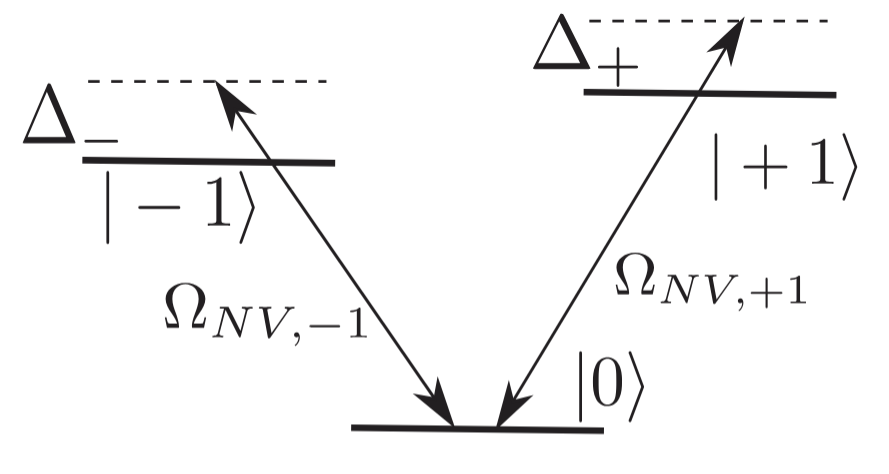
\includegraphics[width = 0.5\linewidth]{/home/hawk/desktop/lab/papers/src/Large_quantum_superpositions_of_a_levitated_nanodiamond_through_spin-optomechanical_coupling/1b.png}
    \end{figure}
    系のハミルトニアンは,
    \begin{align}
      \hat{H}_{\r{eff}} = \hbar\omega_{\r{m}}\hat{a}^{\dag}_{\r{m}}\hat{a}_{\r{m}} + \hbar\Omega\hat{\sigma}_z + \hbar\lambda\qty(\hat{\sigma}_+ + \hat{\sigma}_-)\qty(\hat{a}_{\r{m}} + \hat{a}^{\dag}_{\r{m}})
    \end{align}
    となる.
    \par
    また,マイクロ波を切ると系のハミルトニアンは,
    \begin{align}
      \hat{H} = \hbar\omega_{\r{m}}\hat{a}^{\dag}_{\r{m}}\hat{a}_{\r{m}} + \hbar\lambda\qty(\hat{\sigma}_+ + \hat{\sigma}_-)\qty(\hat{a}_{\r{m}} + \hat{a}^{\dag}_{\r{m}})
    \end{align}
    となる.
    また,マイクロ波を切る前と切った後でトラップの周波数を$\omega_{\r{m}} = \omega_{\r{m}1}$から,$\omega_{\r{m}} = \omega_{\r{m}2}$へと変化させる.
    このとき,系の時間発展により$T_2 / 2 = \pi / \omega_{\r{m}2}$では,
    \begin{align}
      \ket{\Phi_{\pm}}_{n} = \frac{1}{\sqrt{2}}\qty(\ket{+1}\ket{D_m / 2}_{n} + \ket{-1}\ket{-D_m / 2}_{n})
    \end{align}
    となる.
    これでは,もつれた猫状態であり,もつれを解消する.
    $\ket{+1}\ket{D_m / 2}$と$\ket{-1}\ket{-D_m / 2}$の間のエネルギー差は$2.4\ \r{MHz}$であるのに対して,$\ket{+1}$と$\ket{-1}$の間のエネルギー差は$\r{kHz}$オーダーであるので,
    選択的に$\ket{1}\ket{D_m / 2}$から$\ket{0}\ket{D_m / 2}$へと変化させることができる.
    同様に,$\ket{-1}\ket{D_m / 2}$から$\pm\ket{0}\ket{D_m / 2}$へと変化させることができる.
    なぜこれに複号が付くのかわからない.
    そのときは,
    \begin{align}
      \ket{\psi_{\pm}}_n = \frac{1}{\sqrt{2}}\qty(\ket{D_m / 2}_{n} \pm \ket{-D_m / 2}_{n})
    \end{align}
    \par
    なお,振動の測定には量子非破壊測定を行う.
    そのハミルトニアンは,
    \begin{align}
      \hat{H}_{\r{QND}} = \hbar\chi\hat{\sigma}_z\hat{a}^{\dag}_{\r{m}}\hat{a}_{\r{m}}
    \end{align}
    である.
    NVのスピンを,
    \begin{align}
      \ket{\psi}_{\r{measure}} = \frac{1}{\sqrt{2}}\qty(\ket{+} + \e^{\i\phi}\ket{-})
    \end{align}
    と準備して,$\hat{H}_{\r{QND}}$で時間発展させると,相対位相は,
    \begin{align}
      \phi(t) = \phi(0) + 2\chi nt
    \end{align}
    と時間発展するので振動非破壊測定できる.
  \section{結果}
    \begin{figure}[H]
      \centering
      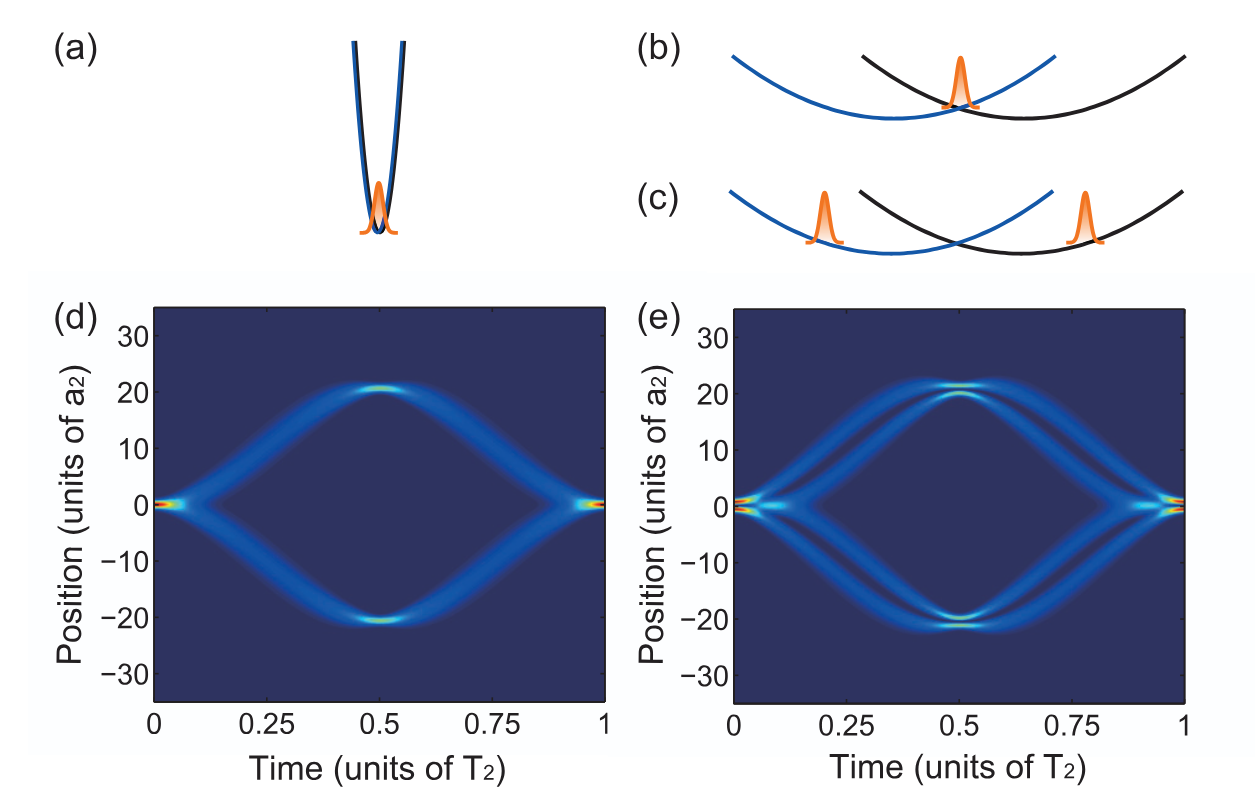
\includegraphics[width = 0.5\linewidth]{/home/hawk/desktop/lab/papers/src/Large_quantum_superpositions_of_a_levitated_nanodiamond_through_spin-optomechanical_coupling/3.png}
    \end{figure}
    (a)は最初に基底まで冷却したときである.
    (b)と(c)はマイクロ波を切ったときの波動関数の広がり,(d)は運動の初期状態を$\ket{0}$としたとき,(e)は運動の初期状態を$\ket{1}$としたときである.
    \begin{figure}[H]
      \centering
      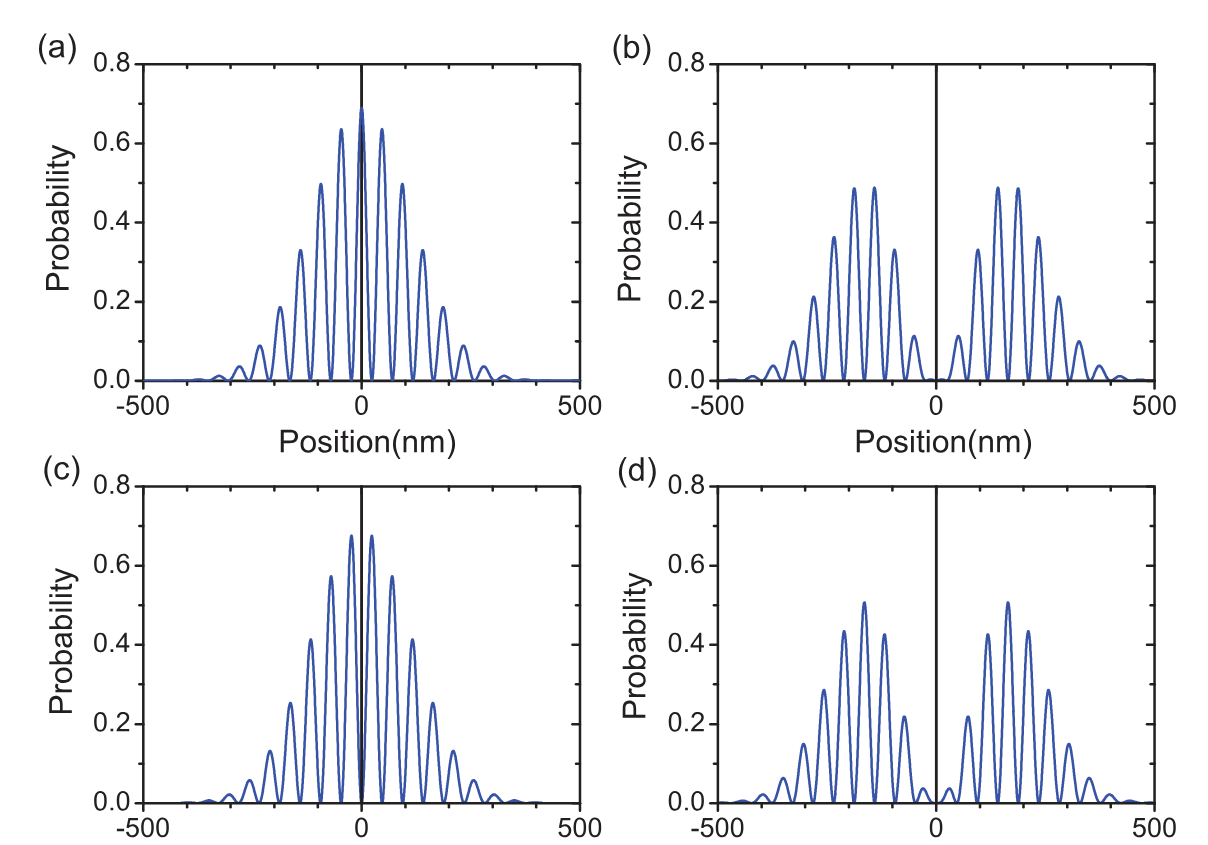
\includegraphics[width = 0.5\linewidth]{/home/hawk/desktop/lab/papers/src/Large_quantum_superpositions_of_a_levitated_nanodiamond_through_spin-optomechanical_coupling/5.png}
    \end{figure}
    エンタングルした状態を変えながら位置ごとの存在確率を表した図.
    順に,$\ket{\psi_{+}}_0$,$\ket{\psi_{+}}_1$,$\ket{\psi_{-}}_0$,$\ket{\psi_{-}}_1$である.
    \begin{figure}[H]
      \centering
      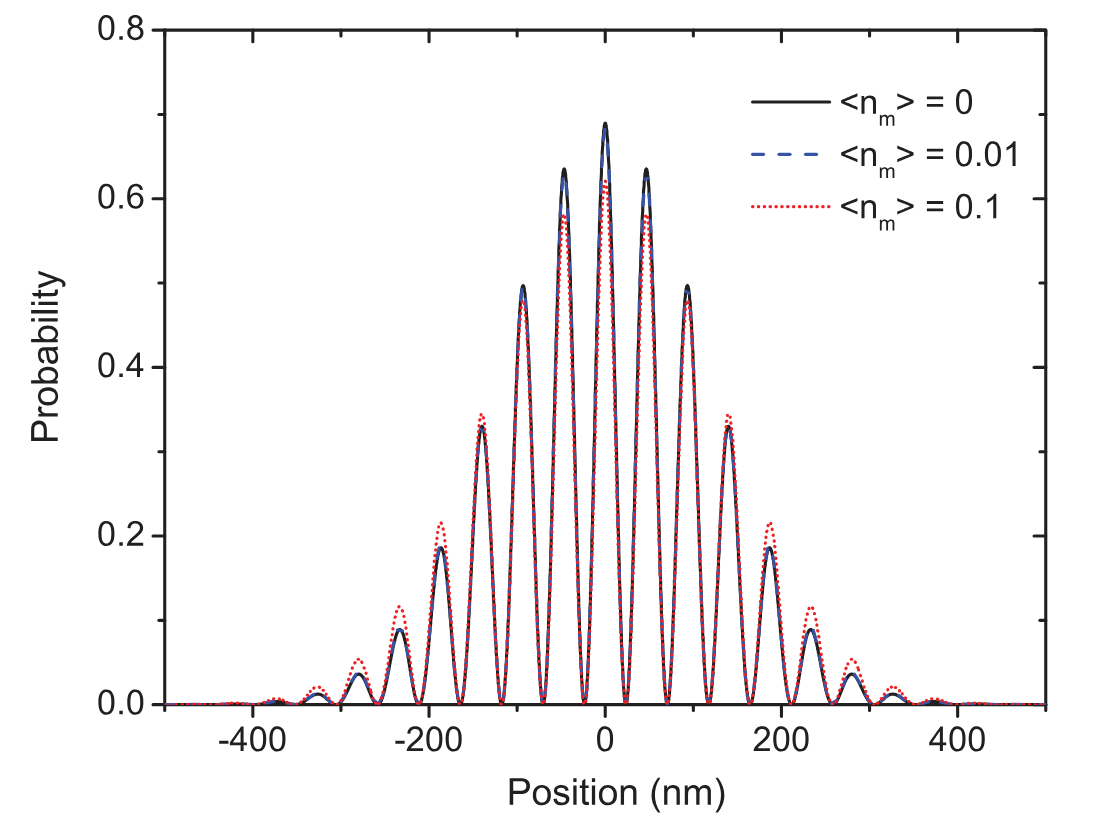
\includegraphics[width = 0.5\linewidth]{/home/hawk/desktop/lab/papers/src/Large_quantum_superpositions_of_a_levitated_nanodiamond_through_spin-optomechanical_coupling/6.png}
    \end{figure}
    熱による緩和を入れたときの図.
    $\ev{n} \ll 1$のとき,熱に対して運動状態はロバストである.
\end{document}